\documentclass[]{report}
\usepackage{graphicx}
\usepackage{geometry}
 \geometry{
 a4paper,
 total={170mm,257mm},
 left=20mm,
 top=20mm,
 width=17cm,
 }
\usepackage{ragged2e}

\begin{document}
\begin{center}
 {\Large Data Intensive Computing - Review Questions 2}
 \end{center}
 \begin{center}
 {\small Daniele Montesi, Francesco Staccone}
 \end{center}
 \vspace{1cm}
\justify
\begin{enumerate}
 \item Imagine you are working in a big company, and your company is planning to launch the next big Blogging platform. Tomorrow morning you go to your office and see the following mail from your CEO regarding a new work. How do you answer to this email? Hint: use MapReduce to solve it, and explain what you do in Map and Reduce phases. \\
  \begin{verbatim}
  Dear Francesco&Daniele,
  As you know we are building a blogging platform, and I need some statistics. 
  I need to find out, across all blogs ever written on our blogging system, how many 
  times 1 character words occur (e.g., "a", "I"), How many times two character words 
  occur (e.g., "be", "is"),  and so on.
  I know its a really big job.  I am going on a vacation for one week, and its really 
  important that I’ve this when I return.
  Good luck.
  Regards,
  The CEO
   \end{verbatim}
The text collected across all the blogs is used as input data for the MapReduce procedure. The input text is divided into fixed-size pieces called input splits, each of which is consumed by a single mapper. In our case, the aim of the Map phase is to count the number of letters in each word from input splits and prepare a key-value list in the form of (n.of letters, 1). In the Shuffle phase, then, emitted (key, value) pairs are grouped together according to their keys and passed to a single machine, which runs the Reduce script over them. Output values from the Shuffle phase are aggregated counting the number of words with the same amount of letters, so that we can get their frequencies as final output of the Reduce phase. \\
 
 \item Briefly explain the differences between Map-side join and Reduce-side join in Map-Reduce?\\\\
 Join is an operation used to combine two or more database tables based on foreign keys. In Map-Reduce, the join is classified into two types depending on where it is actually performed:\\

1. \textbf{Map-side join} is when join is performed by the Mapper, before that data are actually consumed by the map function. To let that happen, the input to each map function must be in the form of a partition and in sorted order. It is also mandatory to have an equal number of partitions, sorted by the join key. In the scenario in which one of the tables is small, a MapReduce local task is created before the original join MapReduce which reads data of the small table from HDFS and stores it into an in-memory hash table. Then, the in-memory hash table is serialized into a hash table file. Now, when the original MapReduce join task runs, data are moved from the hash table file to the \textit{Hadoop distributed cache} that populates the local disk of the mappers, each of which can load this persistent hash table file back into the memory and do the join task as before.  This procedure is adequate only when one of the tables is small enough to fit into the memory, so that it can be read just once. In this case, Map-side join minimizes the costs related to sorting and merging in the shuffle and reduce stages, improving the performance of the task.\\

2. \textbf{Reduce-side join}, when it is performed by the Reducer. Here there is no need here to have a dataset in a partitioned form: the join operation can be performed on unstructured data as well. The map function emits join key and corresponding tuples of both the tables. As a result of this processing, all the records with same join key reach the same reducer which then joins them. Compared to the Map-side join, it is easier to implement since we can take advantage of the inbuilt sorting and shuffling algorithm in the MapReduce framework that sends the values having identical keys to the same reducer, therefore data are already organized. On the other hand, the Reduce-side join  generates a huge network I/O traffic in the sorting and reducer phase, thus there is chance to encounter an OutOfMemory Exception in case of a large number of different datasets with millions of values.\\\\


 
 \item Explain briefly why the following code does not work correctly on a cluster of computers. How can we fix it?
  \begin{verbatim}
  val uni = sc.parallelize(Seq(("SICS", 1), ("KTH", 2)))
  uni.foreach(println)
 \end{verbatim}
 The aforementioned code does not work properly on a cluster of computers because in Spark the \textit{foreach} operation is an action that is performed on each cluster separately and \textbf{does not collect} data back to the Driver. Thus, in this case the \textit{println} is executed on each of the workers, that will print their own RDD partition data instead of returning the RDD values to the Driver.\\ To fix the problem I can use a \textbf{collect()} action to let the code behave as desired, collecting the data on the Driver: \\

 \begin{verbatim}
   val uni = sc.parallelize(Seq(("SICS", 1), ("KTH", 2)))
   uni.collect().foreach(println)
 \end{verbatim}
 

 
 \item Assume you are reading the file campus.txt from HDFS with the following format:\\
\textit{  SICS CSL\\
  KTH CSC\\
  UCL NET\\
  SICS DNA\\
  ...\\}
Draw the lineage graph for the following code and explain how Spark uses the lineage graph to handle failures.
\begin{verbatim}
val file = sc.textFile("hdfs://campus.txt") 
val pairs = file.map(x = (x.split(" ")(0), x.split(" ")(1))) 
val groups = pairs.groupByKey()
val uni = sc.parallelize(Seq(("SICS", 1), ("KTH", 2)))
val joins = groups.join(uni)
val sics = joins.filter(x = x.contains("SICS"))
val list = sics.map(x = x.\_2)
val result = list.count
\end{verbatim}

The following graph represents the lineage of the above Scala code.
\begin{center}
  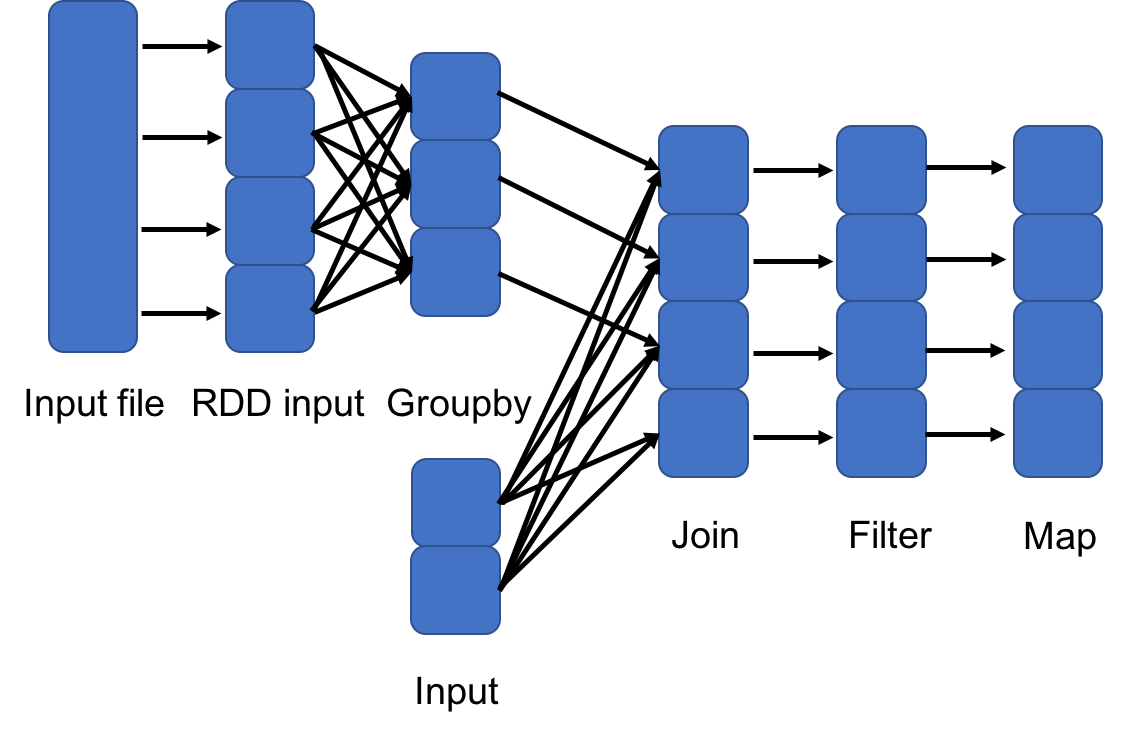
\includegraphics[width=0.5\textwidth]{Lineage.png}\\
  Figure 1: lineage graph
\end{center}

Spark is able to handle failure very efficiently thanks to the Lineage graph, which is used to recompute lost partitions.\\ This graph stores all the information on the operations applied on the input data. This happens thanks to an interface based on coarse-grained transformations i.e. they apply the same operations to more splits, allowing to log the transformation itself on the lineage. 
Thus, it is possible to recompute only the partitions of data that fail starting from the failing partition and back tracking it in a lineage graph, avoiding to write all RDDs/Data to the disk. 
\end{enumerate}


\end{document}
